\documentclass[a4paper, 10pt, oneside]{memoir}
\usepackage{style}

\usepackage{animate}
\usepackage{wrapfig}
%\usepackage{import}
\usepackage{subfiles}

% ТИТУЛЬНИК
\title{
\vspace{4cm}
\normalfont \normalsize 
\horrule{0.5pt} \\[0.4cm]
\huge Конспект по обучению с подкреплением
\horrule{2pt} \\[0.5cm]
}

\author{Издание дописанное и доработанное}

\date{\normalsize\today}

\begin{document}
% Делаем мат. формулы жирными! 
\mathversion{bold}

% Вставляем титульник
\maketitle
\thispagestyle{empty}

% Роботы
\begin{center}
    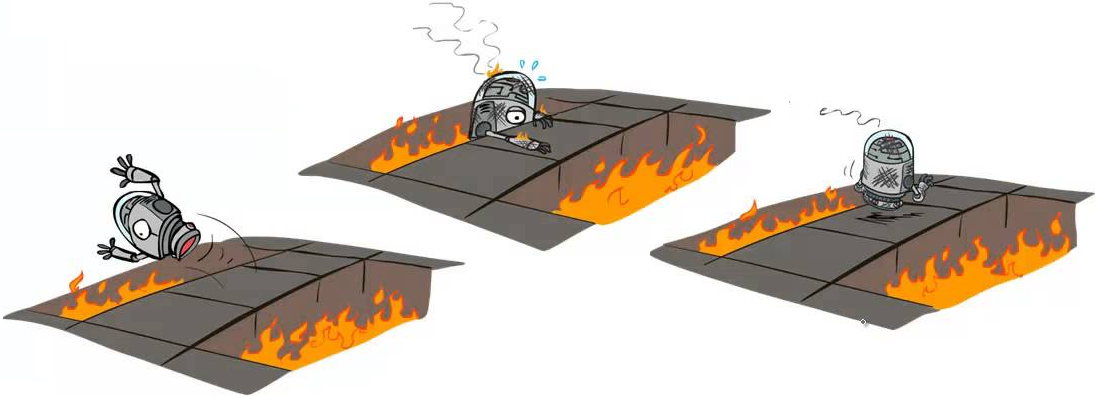
\includegraphics[width=0.7\textwidth]{Images/robot.png}
\end{center}

% Дисклеймер
\vspace{2cm}
\begin{center}
\textcolor{ChadBlue}{\underline{\textbf{Дисклеймер}}}
\end{center}

\vspace{0.75cm}
В этом конспекте собрана теория по глубокому обучению с подкреплением из разных источников. Предпринята отчаянная попытка как-то унифицировать ход рассуждений, обозначения и определения, а также соблюсти тонкий баланс между строгостью и понятностью изложения. В тексте и в доказательствах потенциально присутствует откровенная лажа; \textbf{соответственно, просьба всем читателям собирать все опечатки, баги, вероятные ошибки, несогласованные обозначения и просто вызвавшие недоумение моменты} и отправлять в любом виде мне.

\newpage
\begin{center}
\textcolor{ChadBlue}{\underline{\textbf{Обозначения}}}
\end{center}

\vspace{0.5cm}
От читателя предполагается знание базовой теории вероятности (условная вероятность, формула Байеса, правило суммы и произведения), основ машинного обучения, глубокого обучения и векторного дифференцирования. 

Будут использоваться обозначения $\E$ для математических ожиданий и $\Prob(A)$ для вероятностей события $A$. Если некоторое распределение задано с точностью до нормировочной константы, будем писать $p(a) \propto f(a)$, тогда нормировочная константа может быть вычислена как $\int f(a) \diff a$. \href{https://ru.wikipedia.org/wiki/\%D0\%A0\%D0\%B0\%D1\%81\%D1\%81\%D1\%82\%D0\%BE\%D1\%8F\%D0\%BD\%D0\%B8\%D0\%B5_\%D0\%9A\%D1\%83\%D0\%BB\%D1\%8C\%D0\%B1\%D0\%B0\%D0\%BA\%D0\%B0_\%E2\%80\%94_\%D0\%9B\%D0\%B5\%D0\%B9\%D0\%B1\%D0\%BB\%D0\%B5\%D1\%80\%D0\%B0}{Дивергенцию Кульбака-Лейблера} между двумя распределениями $p(x)$ и $q(x)$ будем обозначать $\KL(p(x) \parallel q(x))$.

Параметрические функции (под которыми обычно будут подразумеваться нейронные сети) $f$ со входом $x$ с параметрами $\theta$ будут обозначаться как $f(x, \theta)$ или как $f_{\theta}(x)$; если моделируется распределение, то будут использоваться записи $p(y \mid x, \theta)$ или $p_\theta(y \mid x)$. В процессах оптимизации по $\theta$ мы будем обозначать константные (не зависящие от параметров $\theta$) слагаемые как $\const(\theta)$.

\begin{remark}
Орешком будут обозначаться некоторые заметки автора о некоторых инженерных и практических трюках обсуждаемых алгоритмов. Например: обычно для обучения нейросетей в RL используют метод \href{https://arxiv.org/abs/1412.6980}{Adam}.
\end{remark}

% Вставляем оглавление
\newpage
\tableofcontents*

% Поехали!
\subfile{1.Setup/1. Chapter.tex}
\subfile{2.MetaHeuristics/2. Chapter.tex}
\subfile{3.ClassicTheory/3. Chapter.tex}
\subfile{4.ValueBased/4. Chapter.tex}
\subfile{5.PolicyGradient/5. Chapter.tex}
\subfile{6.ContinuousControl/6. Chapter.tex}
\subfile{7.ModelBased/7. Chapter.tex}
\subfile{8.NextStage/8. Chapter.tex}

\vspace{2cm}
\begin{center}
That's all, folks!
\end{center}

\newpage

\appendix

\chapter{Приложение}

\import{Appendix/}{NaturalGradient.tex}
\import{Appendix/}{QLearningConvergence.tex}

%END PAGE-----------------------------------------------
\import{}{sources.tex}

\newpage
\thispagestyle{empty}
\begin{center}
\vspace*{5cm}

\includegraphics[width=10cm]{Images/reach.jpg}
\end{center}
\end{document}